
\section{Deep Dive Computer Science Part}
\subsection{Understanding ipykernel}
\subsubsection{Overview Python Interpreter}
Reference: \href{https://docs.python.org/3/tutorial/interpreter.html#the-interpreter-and-its-environment}{Using the Python Interpreter}, \href{https://blog.hubspot.com/website/what-is-python-interpreter#:~:text=A%20python%20interpreter%20is%20a,and%20low%2Dlevel%20languages%20are.}{What Is a Python Interpreter?}\\


\paragraph{High-Level Language}
The \gls{g_Python} language is a high-level programming language. This means, that the programming language is more similar to human language then to machine language, which is written in strings of bits - ones and zeros.
The advantage of it is that it is better understood by humans, but the same can not be said for the machines. Writing commands (instruction) in lines of zeros and ones is more difficult, that using higher level concepts. The gap between this, gets closes by the \textbf{Python Interpreter}.\\

The \gls{g_PyI} reads the command written by the \gls{g_Python} programmer, evaluates them, and returns the output. If the \textit{python.exe} application/ interpreter is opened, either through the \gls{CMD}, for example  
\begin{lstlisting}[language=iCMD]
	$ python3.12
	///Python 3.12 (default, April 4 2022, 09:25:04)
	///[GCC 10.2.0] on linux
	///Type "help", "copyright", "credits" or "license" for more information.
	>>>
\end{lstlisting}
the commands
\begin{lstlisting}[language=iCMD]
	>>> the_world_is_falt = True
	>>> if the_world_is_flat:
			print("Be careful not to fall off!")
	/// Be careful not to fall off!
\end{lstlisting}
or by opening the application directly.
\begin{figure}[H]
	\centering
	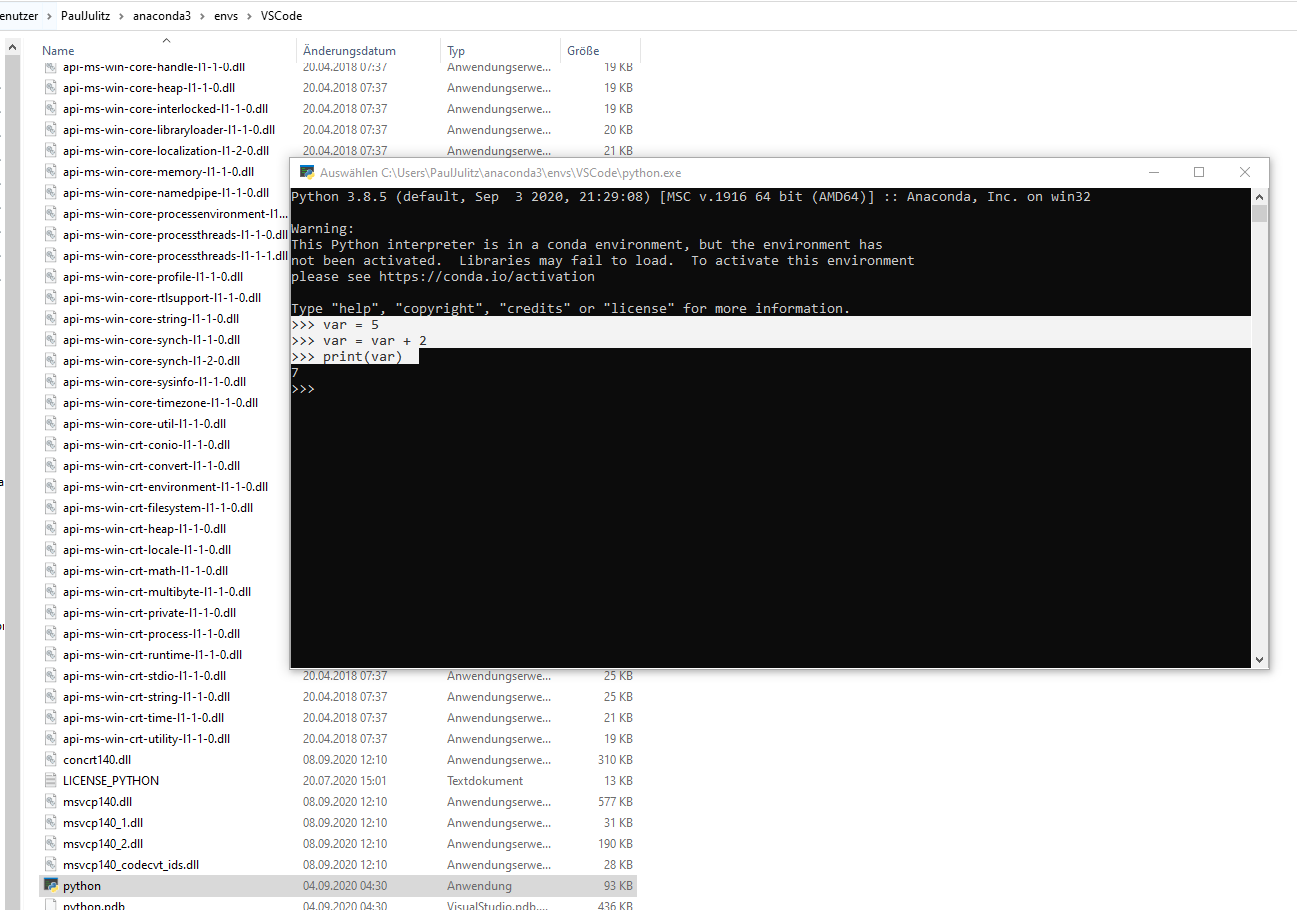
\includegraphics[scale = 0.2]{attachment/chapter_AML/Scc003}
	\caption{Using the command line with the python application/ interpreter}
\end{figure}
In both cases, the \gls{g_PyI} receives the commands and executes them. In the case where the \gls{IDE} is to write a the Python script (aka. module or application), the scripts gets passed to \gls{g_PyI}.\\

\paragraph{Difference between interpreter and a compiler}
Both the interpreter and compiler transforms the source code into binary machine code.
The difference arise through the way they are doing it differently: The interpreter translate the source code one statement at a time. The compiler on the other hand first scans the entire programm and then translate the whole program into machine code. For more detail, see \href{https://blog.hubspot.com/website/what-is-python-interpreter#:~:text=A%20python%20interpreter%20is%20a,and%20low%2Dlevel%20languages%20are.}{What Is a Python Interpreter?} or \href{https://www.analyticsvidhya.com/blog/2021/05/choose-best-python-compilers-for-your-machine-learning-project-detailed-overview/#:~:text=What%20is%20a%20Python%20compiler,executed%20directly%20by%20a%20computer.}{Best Python Compiler}
\begin{figure}[H]
	\centering
	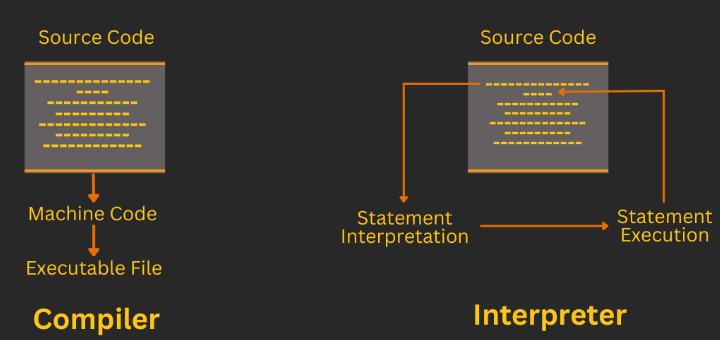
\includegraphics[scale = 0.3]{attachment/chapter_AML/Scc004}
	\caption{Example Compiler and Interpreter in Java}
\end{figure}

\subsubsection{ipykernel (Jupyter Notebook)}
Reference: \href{https://www.reddit.com/r/learnprogramming/comments/imhxai/what_is_the_difference_between_a_python_kernel_as/#:~:text=Python%20kernel%20is%20just%20a,is%20also%20not%20an%20interpreter.}{Difference Kernel and Interpreter}, \href{https://plotly.com/python/ipython-vs-python/}{IPython vs Python in Python}, \href{https://www.reddit.com/r/learnprogramming/comments/imhxai/what_is_the_difference_between_a_python_kernel_as/#:~:text=Python%20kernel%20is%20just%20a,is%20also%20not%20an%20interpreter.}{reddit:  difference between a Python Kernel (as in Jupyter notebooks) and a Python interpreter (like in PyCharm)?}, \href{https://python-forum.io/thread-40721.html}{jupyter kernel is an interface to the Python interpreter.} 


\paragraph{IPython (Python3)}
To understand the \gls{g_Kernel_Jy_Py} it is helpful to understand \textit{IPython (Notebook)}. The \gls{g_PyI} passes command to it. This only allows commands for \gls{g_Python}.\\


\textit{IPyhton} creates an interactive command line terminal for \gls{g_Python}.  

\begin{figure}[H]
	\centering
	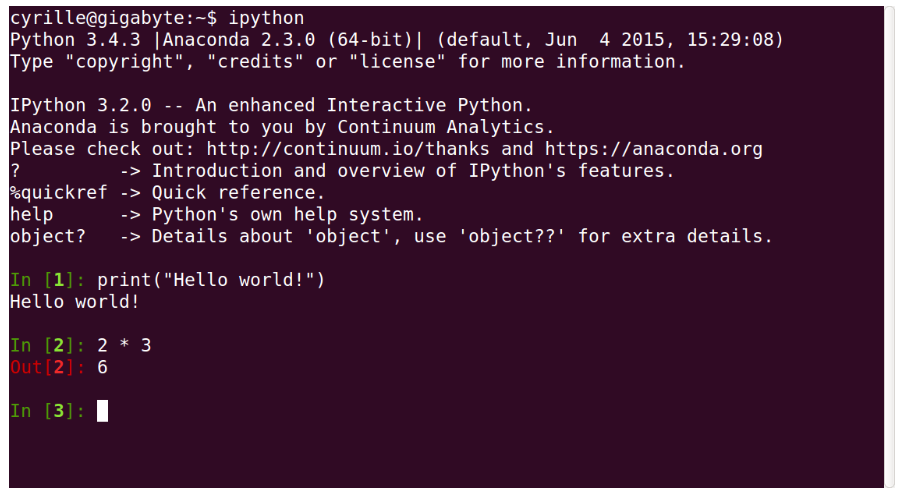
\includegraphics[scale = 0.3]{attachment/chapter_AML/Scc005}
	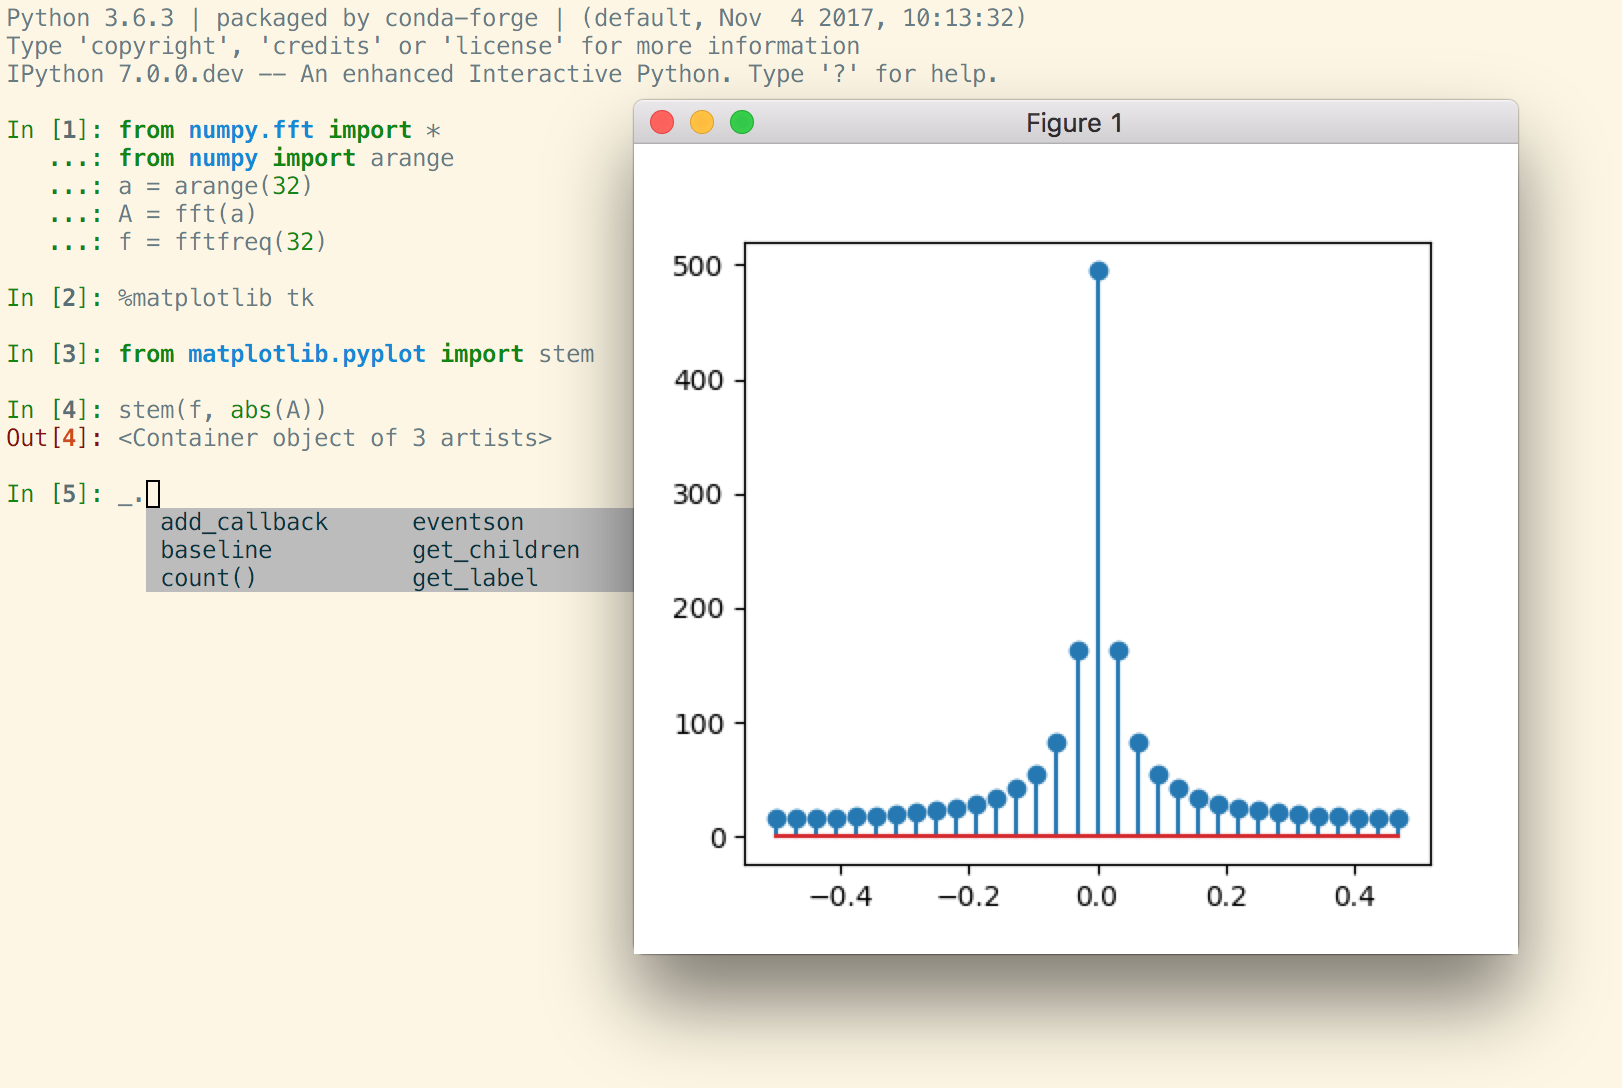
\includegraphics[scale = 0.2]{attachment/chapter_AML/Scc009}
	\caption{IPython interactive command-line terminal}
\end{figure}

\paragraph{Jupyter Notebook}
With the reorganization of \textit{IPython}, the new tool \textbf{Notebook} has been created. Under the project name \textbf{Jupyter}. This \gls{g_JupyterNotebook} is a web interface for \gls{g_Python}. It has the same interactive interface kept. Being a web-interface, it can integrate with many of the existing web libraries for data visualization.\\

The concept of a \textit{kernel} comes into play as the engine behind the web interface. The \textit{IPython} is now the backend with the \gls{g_Kernel_Jy_Py} for \gls{g_Python}. The \gls{g_Kernel_Jy_Py} with the advent of \gls{g_JupyterNotebook} is able to handel \textit{markdown} and \LaTeX text input.\\
\begin{figure}[H]
	\centering
	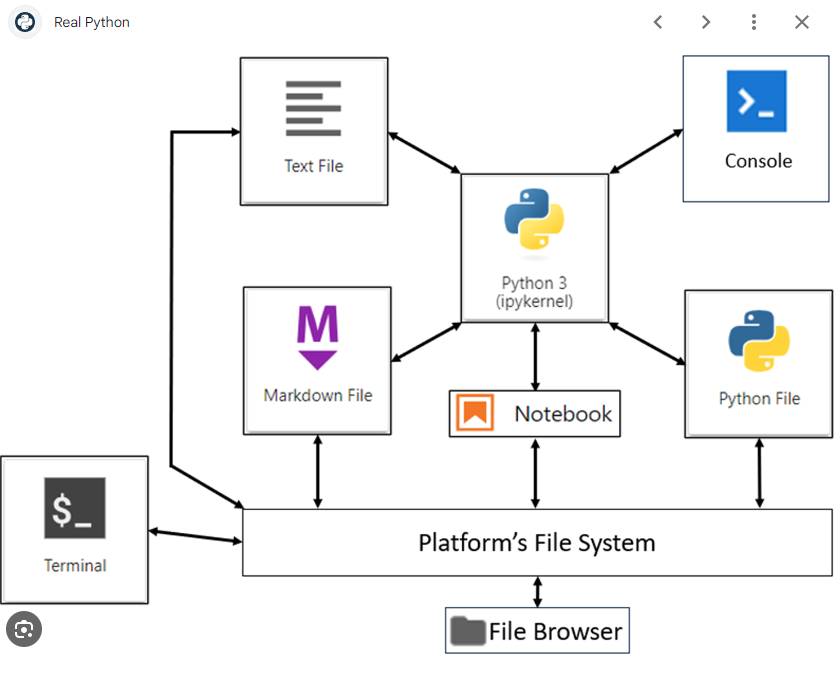
\includegraphics[scale = 0.3]{attachment/chapter_AML/Scc006}
	\caption{JupyterLab for an Enhanced Notebook, \href{https://realpython.com/using-jupyterlab/}{Jupyter Lab}}
\end{figure}
Note: The interaction with the \gls{g_Kernel_Jy_Py} is done through the \gls{g_JupyterNotebook}. With the latest tool: \textbf{Jupyter Lab}, interaction with separate files is possible.\\

$"$Inside$"$ the \gls{g_Kernel_Jy_Py} lives the \gls{g_PyI}. Another way of saying this is that the \gls{g_Kernel_Jy_Py} is the interface to the \gls{g_PyI}.\\

Note: \textit{Jupyter Lab} allows for a more interactive and simultaneous way to code.

\subsubsection{Interacting with different (language) Kernels}
\paragraph{Theoretical Multi languages Kernel}
As said before the \gls{g_Kernel_Jy_Py} is for interacting with the \gls{g_PyI} and the other functionality of a \gls{g_JupyterNotebook}.\\

The community around, \textit{Juypter Notebook}, the application, developed more \gls{g_Kernel_Jy} for the \gls{g_JupyterNotebook}. Those \gls{g_Kernel_Jy} allows to interact with different languages like \textit{Ruby, Scale, R}.\\

It would be possible (Unclear how) to create a \gls{g_Kernel_Jy} which allows to interact with all those languages in one \gls{g_JupyterNotebook}. The current research for this chapter could not found one. For example the \gls{g_Kernel_Jy_Py} allows us to interact for example with \gls{g_Python}, Markdown, Shell Script. This does not conclude for example \gls{SQL}.

\paragraph{VSCode Compute Cells Confusion}
If a \gls{g_JupyterNotebook} is open, for each cell it is possible to select the language for this cell. This those two things. First it changes the \textit{IntelSence} syntax highlights. Secondly, it provides the \gls{g_Kernel_Jy} information about the lanuage which is used in this cell.

\begin{figure}[H]
	\centering
	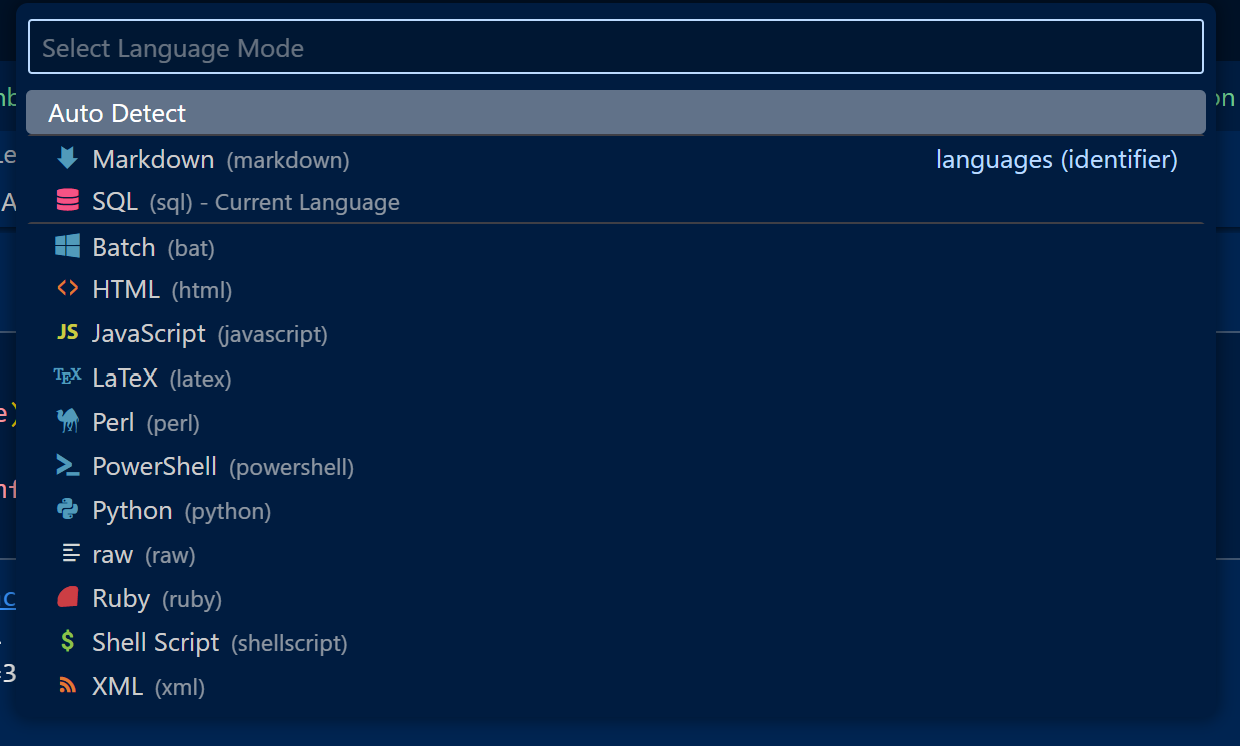
\includegraphics[scale = 0.3]{attachment/chapter_AML/Scc007}
	\caption{Cell Language Mode selection.}
\end{figure}

However, this \underline{does not mean} that all languages are supported by the selected \gls{g_Kernel_Jy}. 

\paragraph{Azure Data Studio}
In Azure Data Studio you can connect to different \gls{g_Kernel_Jy}, \href{
https://learn.microsoft.com/en-us/azure-data-studio/notebooks/notebooks-guidance?view=sql-server-ver15}{Azure Data Studio}:
\begin{itemize}
	\item \gls{SQL} Kernel,
	\item PySpark3 and PySpark Kernel,
	\item Spark Kernel,
	\item Python Kernel (for local development)
\end{itemize}


\subsubsection{VEN and ipykernel}
% Spun up by Jupyter 
% Spn up on your machine
\paragraph{Spinning Up Jupyter Notebook with Anaconda}
\begin{itemize}
	\item First a \gls{g_conda} \gls{VEN} gets created.
	\item The Jupyter Notebook $"$application$"$ gets installed
\end{itemize}
This in turn will install the package for the web interface, \textit{IPython} and the default \gls{g_Kernel_Jy_Py} for \gls{g_Python}.
\begin{lstlisting}[language=iCMD, caption={pip commands to get ready for Jupyter Notebok},captionpos=b]
	pip install jupyter
\end{lstlisting}
This command will import all dependence to work with a \gls{g_Kernel_Jy_Py}. An example of package environment see below.

\begin{lstlisting}[style=CMD, caption={Example Jupyter Notebook conda ven},captionpos=b]
	PS C:\Users\PaulJulitz\iCloudDrive\TexMaker\GitHub_Notizen_DSci\Notizen_DSci> conda list
	# packages in environment at C:\Users\PaulJulitz\anaconda3\envs\VSCode:
	#
	# Name                    Version                   Build  Channel     
	...
	azure-common              1.1.28                   pypi_0    pypi      
	azure-core                1.27.1           py38haa95532_0  
	azure-identity            1.12.0                   pypi_0    pypi      
	azure-keyvault-secrets    4.6.0                    pypi_0    pypi      
	azureml                   0.2.7                    pypi_0    pypi      
	...
	ipykernel                 5.3.4            py38h5ca1d4c_0
	ipython                   7.27.0           py38hd4e2768_0
	ipython_genutils          0.2.0              pyhd3eb1b0_1
	...
	jupyter_client            7.0.1              pyhd3eb1b0_0
	jupyter_core              4.8.1            py38haa95532_0
	jupyter_server            1.4.1            py38haa95532_0
	jupyterlab                3.2.1              pyhd3eb1b0_1
	jupyterlab_pygments       0.1.2                      py_0
	jupyterlab_server         2.8.2              pyhd3eb1b0_0
	...
\end{lstlisting}


\paragraph{Multiple Kernel (Python)}
If the setup is done through the Anaconda interface (\gls{g_conda}). The complete installation is done by Anaconda if the \gls{IDE} \gls{g_JupyterNotebook} is installed. By default \textit{IPython} is installed with the \gls{g_Kernel_Jy_Py}.\\

The command for the installation of the \gls{g_Kernel_Jy_Py} is
\begin{lstlisting}[language=iCMD, caption={pip to install ipykernel},captionpos=b]
	pip install ipykernel
\end{lstlisting}
For example to use \text{Scala}, \href{https://community.databricks.com/t5/data-engineering/how-can-we-run-scala-in-a-jupyter-notebook/td-p/17752}{Link}:
\begin{lstlisting}[language=iCMD, caption={Using Scala for a Notebook},captionpos=b]
	# Install the package
	pip install spylon-kernel
	# To select the kernel in the notebook, create a kernel spec
	python -m spylon_kernel install
	# Start Jupyter Notebook
	ipython notebook
\end{lstlisting}
In the notebook the kernel can be selected. The command is to list the available kernels is
\begin{lstlisting}[language=iCMD, caption={pip to install ipykernel},captionpos=b]
	$ jupyter kernelspec list
	>>>>Available kernels:
	>>>>python2.7        /Users/jakevdp/.ipython/kernels/python2.7
	>>>>python3.3        /Users/jakevdp/.ipython/kernels/python3.3
	>>>>python3.4        /Users/jakevdp/.ipython/kernels/python3.4
	>>>>python3.5        /Users/jakevdp/.ipython/kernels/python3.5
	>>>>python2          /Users/jakevdp/Library/Jupyter/kernels/python2
	>>>>python3          /Users/jakevdp/Library/Jupyter/kernels/python3
\end{lstlisting}
See, \href{https://stackoverflow.com/questions/39007571/running-jupyter-with-multiple-python-and-ipython-paths}{Running Multiple Kernel} for understand how to select a \gls{g_Kernel_Jy} throught the command line.
% English
% for or to?-----
% She studied FOR the exam. "For" indicates the goal, which should be achived.
% She went TO study. "to" indicates the use of a purpose before a infinit verb.

To see which \gls{g_Kernel_Jy} is running, run the following code
\begin{lstlisting}[language=iPython]
	import sys
	print(sys.executable)
	print(sys.version)
	print(sys.version_info)
\end{lstlisting} 

\subsubsection{Connecting a Notebook to a Compute Ressources}
%\paragraph{Locally}
To use a \gls{g_JupyterNotebook}, the web interface creates either a
\begin{itemize}
	\item local server,
	\item or provides the possibility to connect to a Jupyter hosted server.
\end{itemize}
Note: The local server is still your own machine.\\

The packages for connecting to a server are installed in the \gls{VEN}. The "spinning" up is basically the configuration to either a local port on your machine or to a hosted server. The former is used for computing.

\begin{figure}[H]
	\centering
	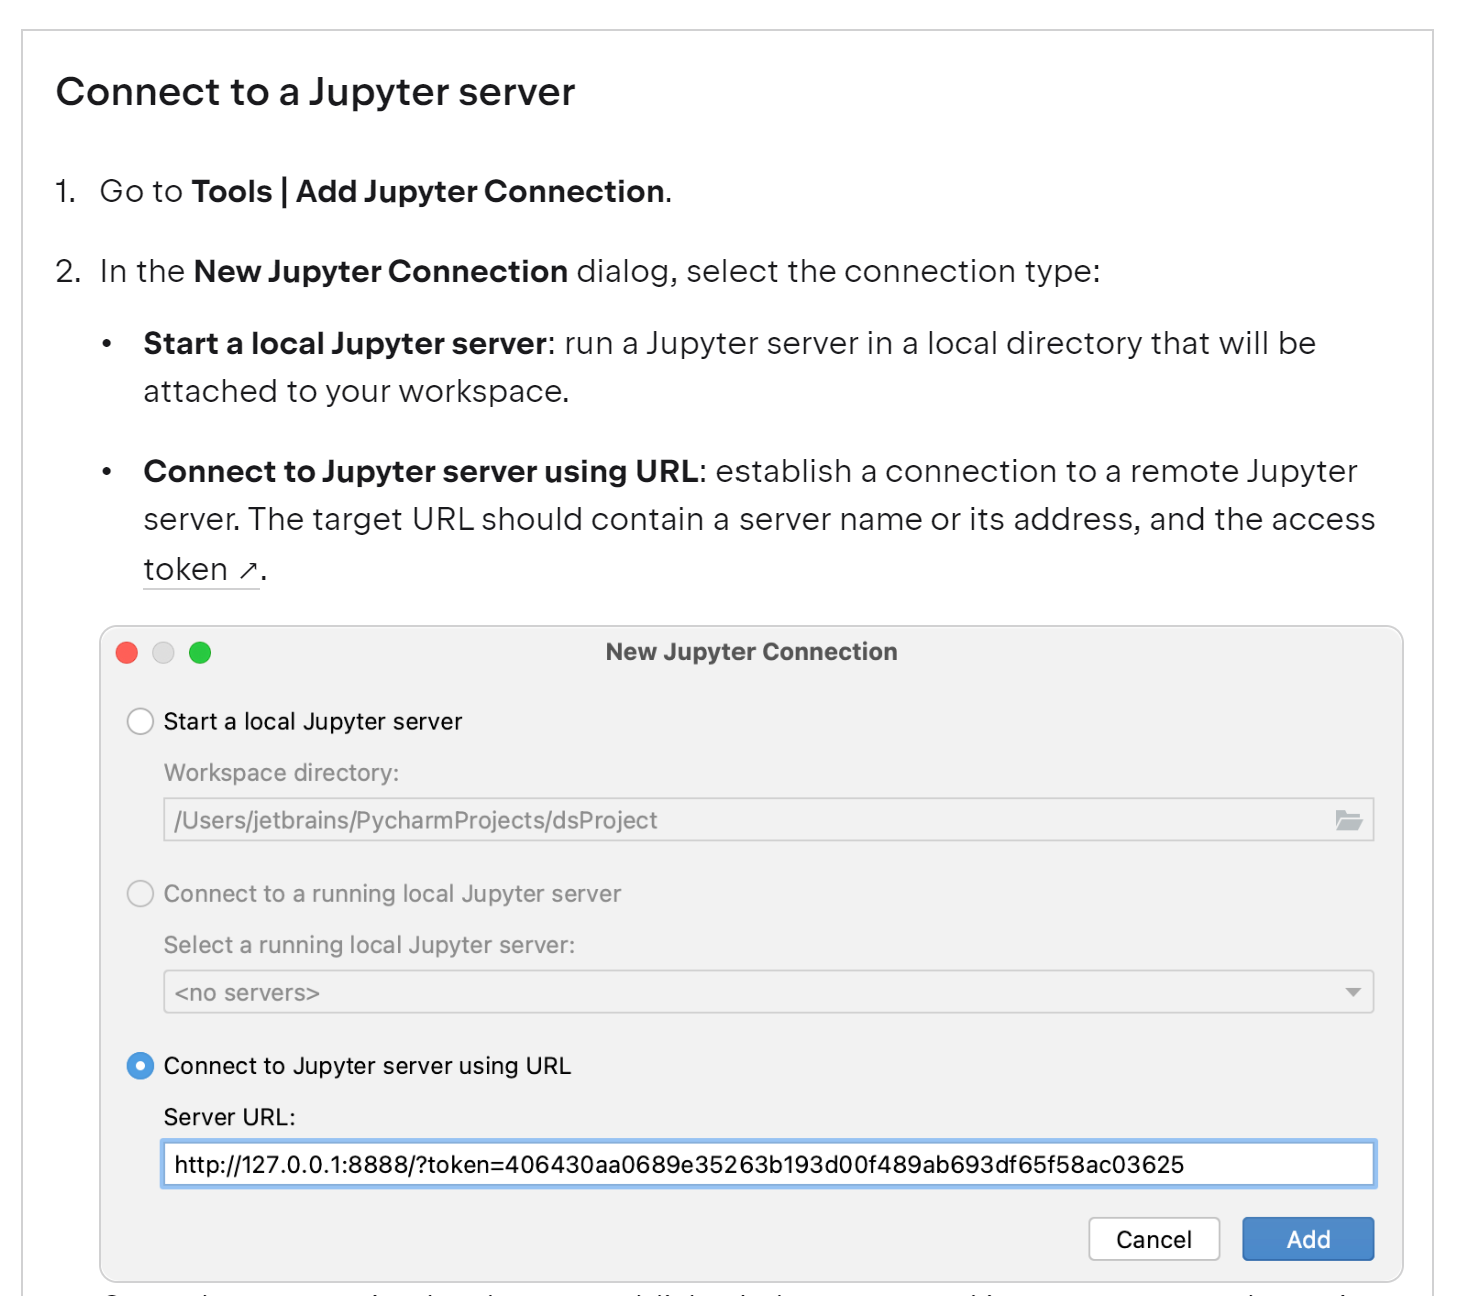
\includegraphics[scale = 0.3]{attachment/chapter_AML/Scc008}
	\caption{Mac Setup of Jupter Notebook Server}
\end{figure}

If the notebook should be connected to the compute cluster, this is done by a SHH Tunnel.

\begin{figure}[H]
	\centering
	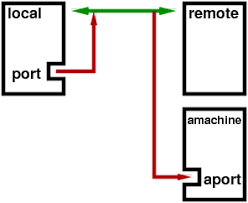
\includegraphics[scale = 0.3]{attachment/chapter_AML/Scc010}
	\caption{Tunnel Trafic, \href{https://radcamp.github.io/AF-Biota/Jupyter_Notebook_Setup.html}{SHH Tunnel}}
\end{figure}

\subsection{Setting Up the Environment}

\subsubsection{Working with conda}
\paragraph{Interacting with conda from the terminal}
Here are three ways to interact with the python interpreter:
\begin{description}
	\item[conda comand] Starting the \textit{Anaconda Navigator} and start the \gls{IDE} from there. This then allows to interact with conda throug the \textbf{conda} \textbf{Cmdlet} from the terminal.
	
	\item[PowerShell Extension] If the local machine has some restriction, that prohibist the use of the command \textbf{conda} from the powershell terminal.
	\begin{figure}[H]
		\centering
		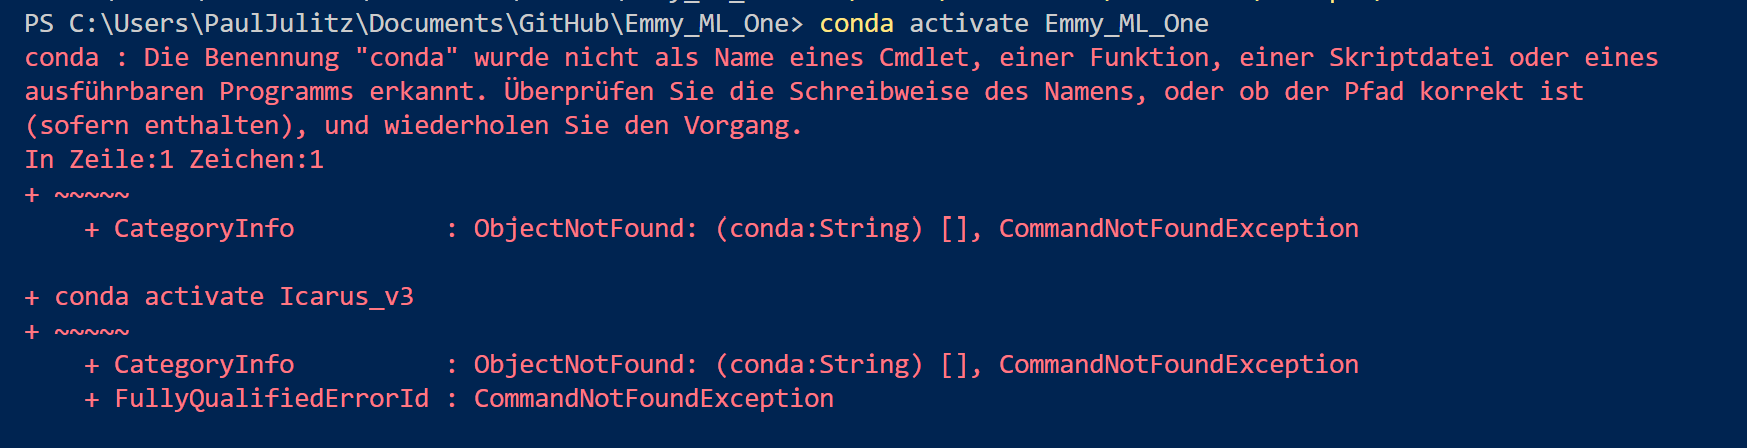
\includegraphics[scale = 0.3]{attachment/chapter_AML/Scc023}
		\caption{Terminal Response by using conda command}
	\end{figure}
	Still, the following powershell script allows when execute to use a \textit{powershell extension}, that bypass this problem.
	\begin{lstlisting}[language=iCMD, caption={.ps1 script}, captionpos=b]
		#region conda initialize
		# !! Contents within this block are managed by 'conda init' !!
		$varPath  = "C:\User\" + (Get-ChildItem Env:USERNAME).Value + "\anaconda\Scripts\conda.exe"
		If (Test-Path $varPath ) {
			(& $varPath  "shell.powershell" "hook") | Out-String | ?{$_} | Invoke-Expression
		}
		#endregion
	\end{lstlisting}
	This powershell extension allows you with the \gls{g_conda} program.
	\begin{figure}[H]
		\centering
		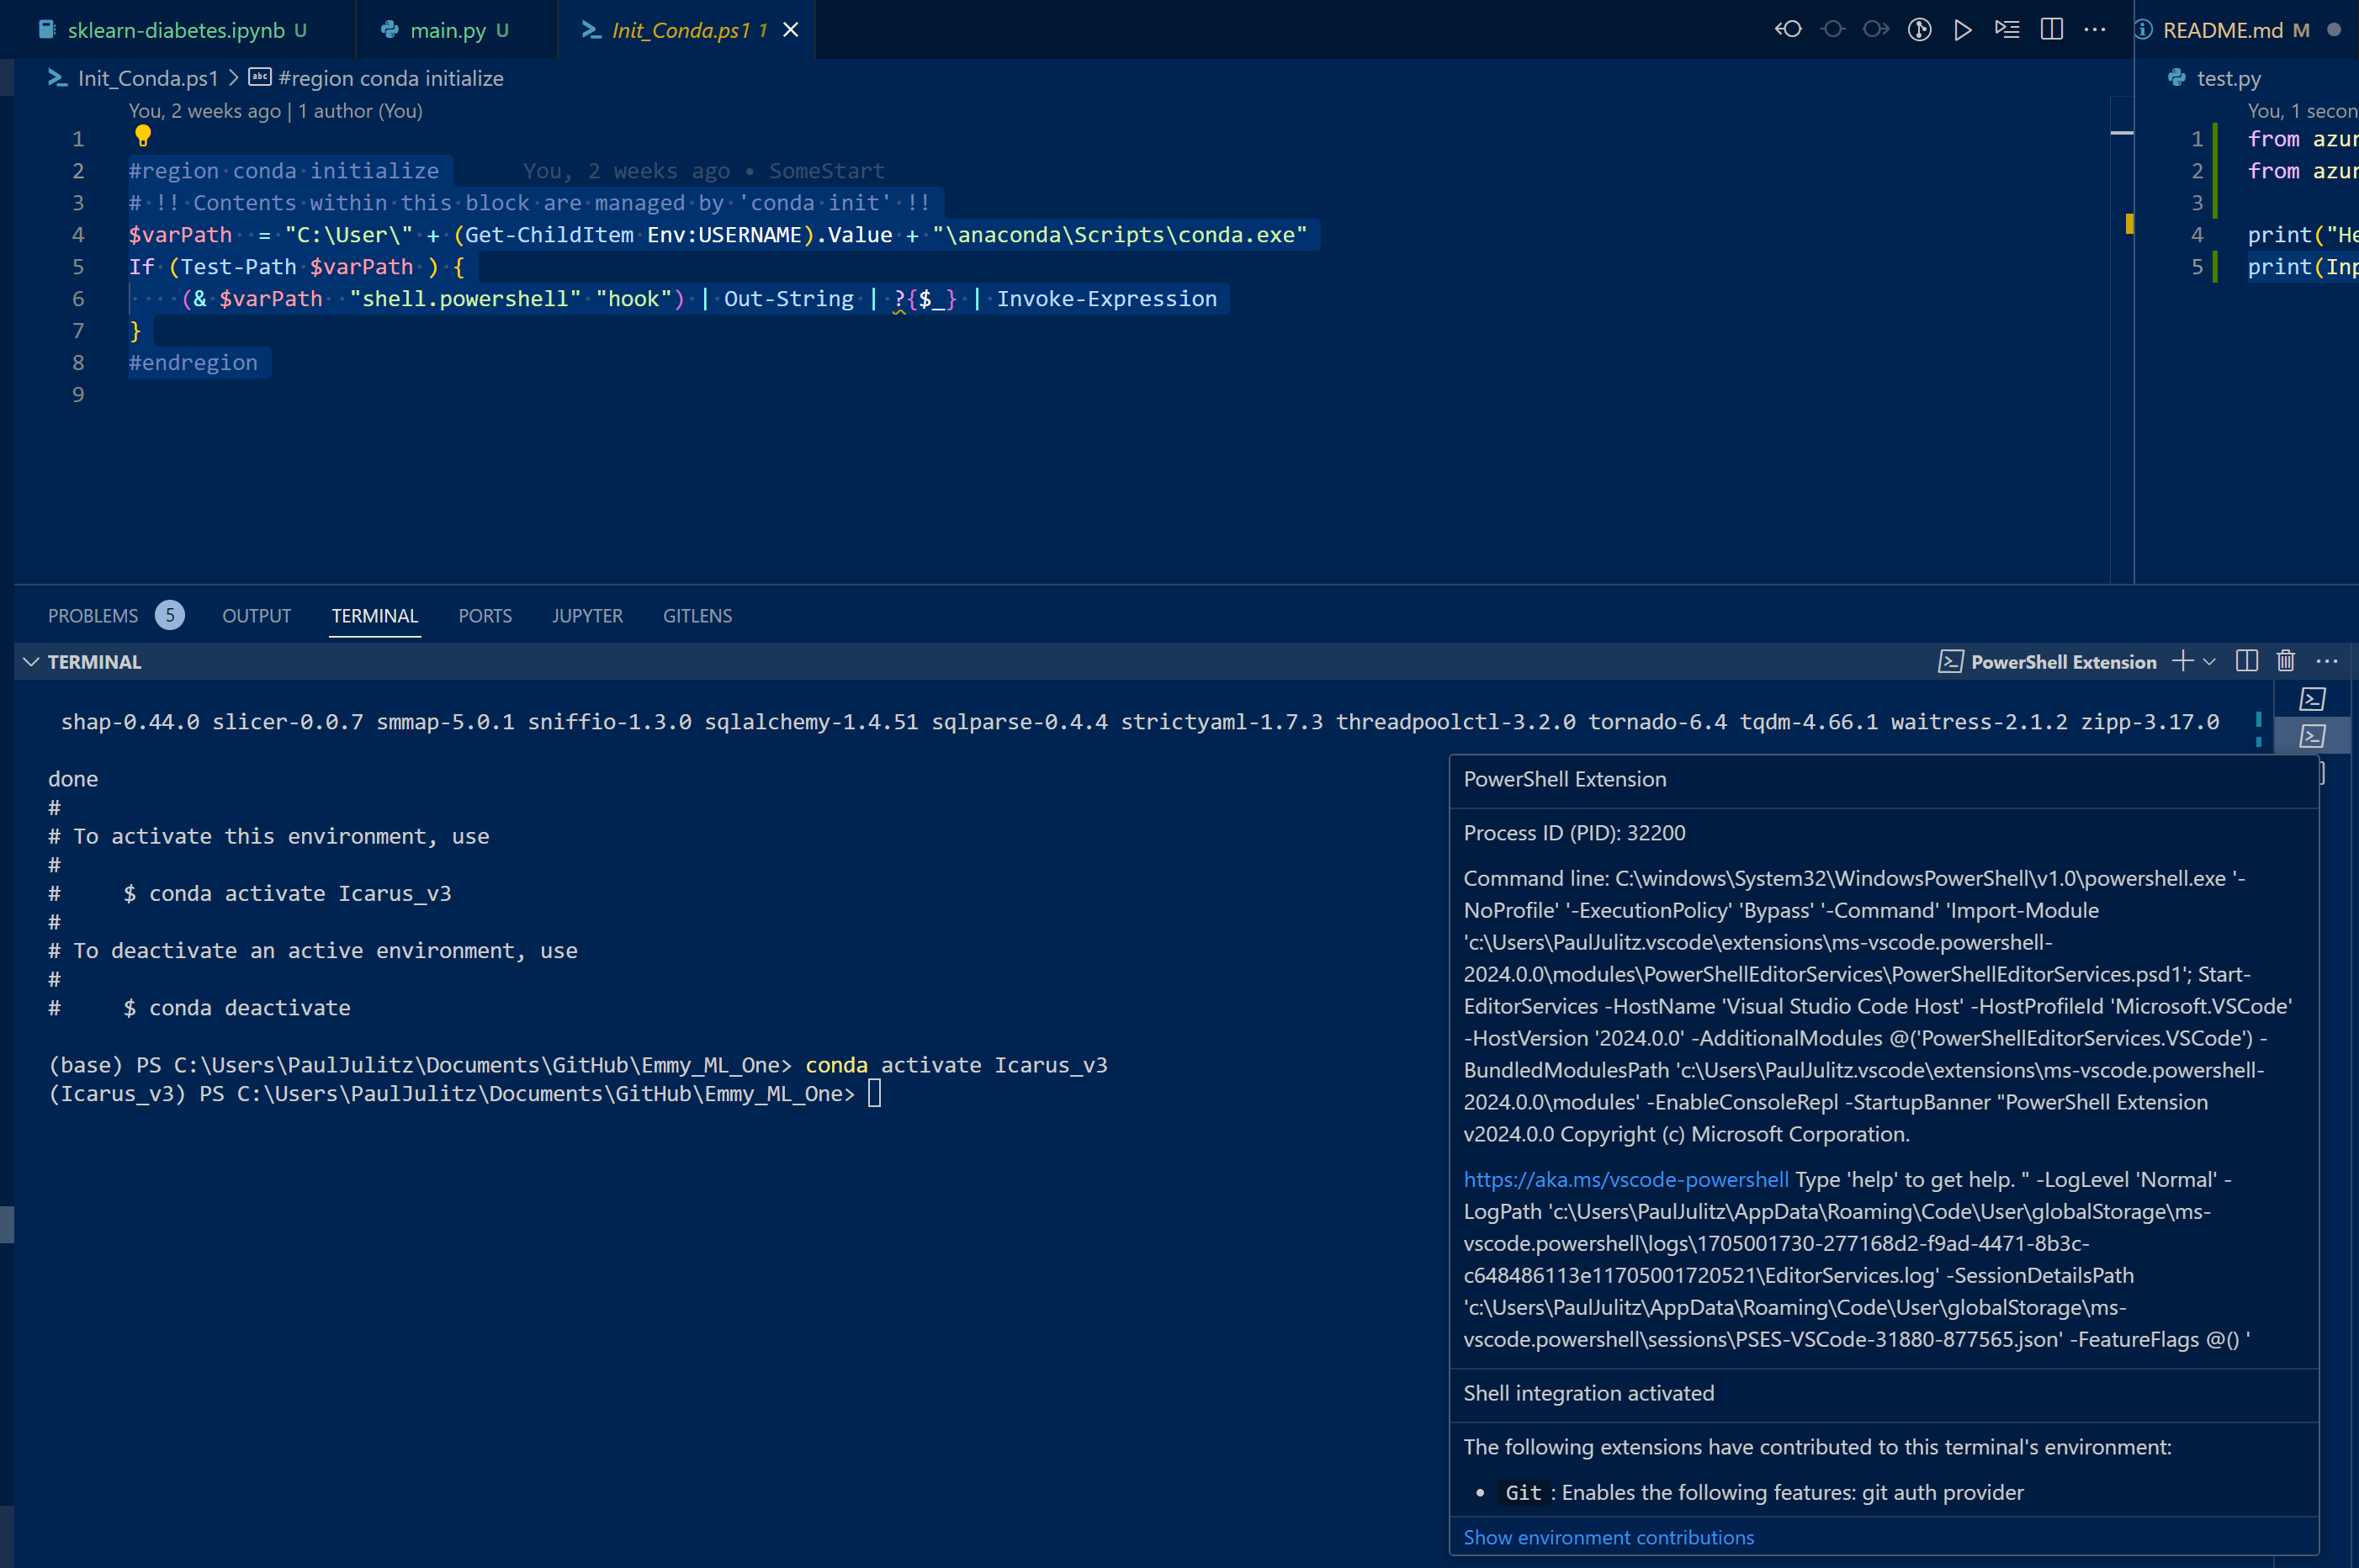
\includegraphics[scale = 0.2]{attachment/chapter_AML/Scc026}
		\caption{PowerShell Extension}
	\end{figure}
	One restriction still exists. In \gls{vsc} the option to run a program requires to create a python terminal in which the \textbf{conda} command can be access. This will not work, because a new terminal will be created in which the \textbf{conda} command can't be access. However, the python interpreter in a specific \gls{g_conda} \gls{VEN} can still be access by providing the direct path to it.
	\begin{figure}[H]
		\centering
		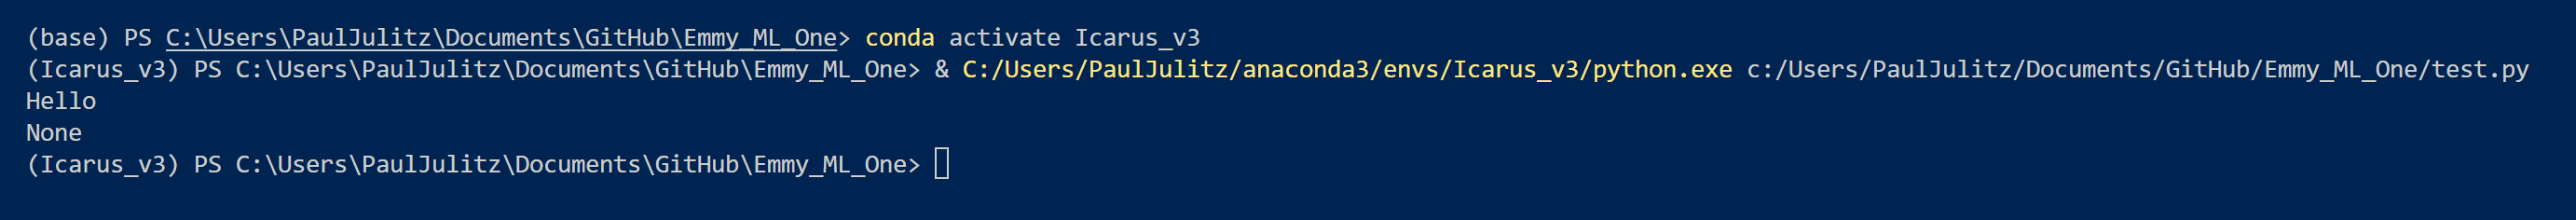
\includegraphics[scale = 0.4]{attachment/chapter_AML/Scc027}
		\caption{PowerShell Extension and Python Interpreter}
	\end{figure}
	\begin{lstlisting}[language=iCMD, caption={Commands}, captionpos=b]
		(base) PS C:\Users\PaulJulitz\Documents\GitHub\Emmy_ML_One> conda activate Icarus_v3
		(Icarus_v3) PS C:\Users\PaulJulitz\Documents\GitHub\Emmy_ML_One> & C:/Users/PaulJulitz/anaconda3/envs/Icarus_v3/python.exe c:/Users/PaulJulitz/Documents/GitHub/Emmy_ML_One/test.py  
		Hello
		None
		(Icarus_v3) PS C:\Users\PaulJulitz\Documents\GitHub\Emmy_ML_One>
	\end{lstlisting}
	\item[Pointing to the interpreter] If the conda command can't be used.
	Then the python interpreter it self can be selected.
	\begin{figure}[H]
		\centering
		
\includegraphics[scale = 0.4]{attachment/chapter_AML/Scc025}
		\caption{Selecting the python interpreter in \gls{vsc}}
	\end{figure}
	Running a python script will use the python interpreter inside the selected \gls{g_conda} \gls{VEN}.
	\begin{figure}[H]
		\centering
		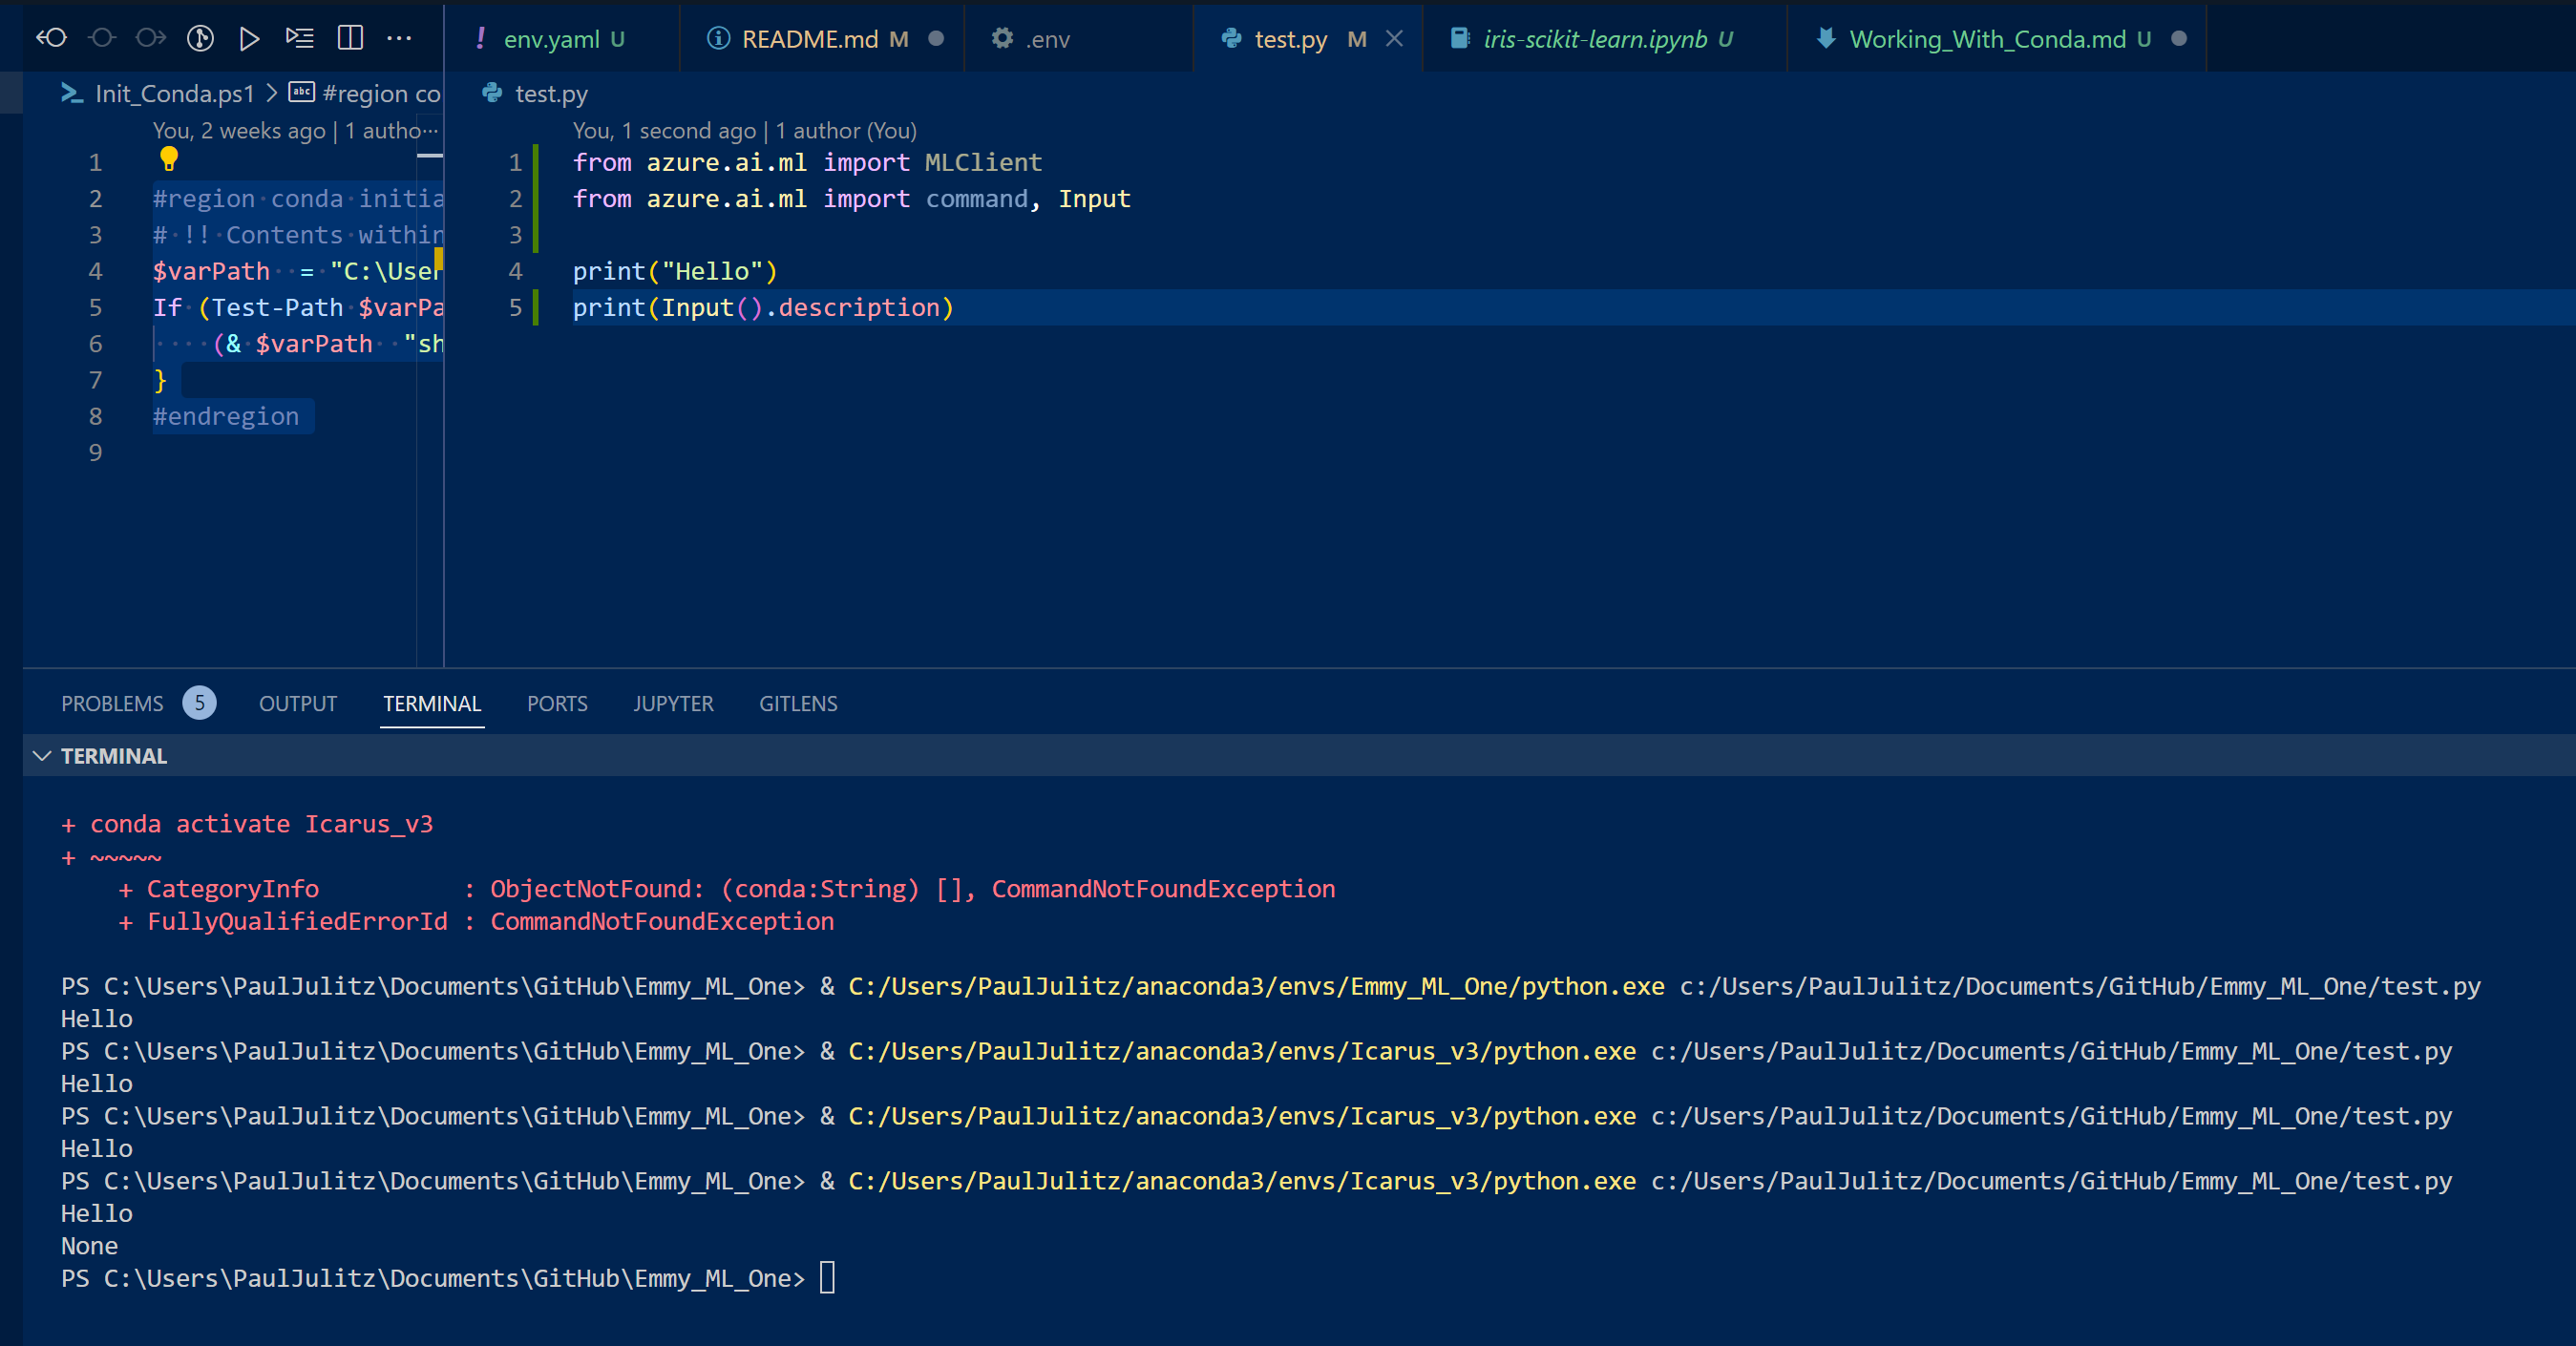
\includegraphics[scale = 0.2]{attachment/chapter_AML/Scc024}
		\caption{Terminal Response by using the python interpreter}
	\end{figure}
\end{description}

\subsubsection{Good Practices for Constants, Configuration and Secrets}
% constant class, see work from Sebastian
% .env is a local file, that allow you to work with secrets and configuration, which you mirrow in the cloud, because you are NOT commiting it.
% setup.sh (Unclear)

\paragraph{.env files (Local Configuration)}
The \textit{.env} has the purpose to store locally secrets and configuration, which are not allowed to commit to the repository. The variable names in his file need to be setup in \gls{CI}/\gls{CD} processes as well, for example in a variable group for a testing pipeline.

\paragraph{Configuration}
To limited scope control a good practices is to store constant in a separate file: : \verb+util/constant.py+.\footnote{See commend out href
	%\href{https://medium.com/@zeid.zandi/how-to-manage-constants-in-python-best-practices-and-advanced-techniques-50fa1591d517#:~:text=Constants%20in%20Python%20are%20typically,access%20and%20modification%2C%20if%20necessary}{How to Manage Constants in Python: Best Practices and Advanced Techniques}
}

Constant defined in a separate file can be imported and accessed from any part of the code base. 


\begin{lstlisting}[language=iPython, caption={Installing Azure ML SDK core package},captionpos=b]
	class Setting:
	"""
	Settings that can be used to change the code behavior.
	"""
	# If False Live paths from configuration.yaml will be used
	TEST_ENVIRONMENT = True
	
	# IF True log  containing already read pvn reports will be deleted so all found pvn files will be used again
	CLEAR_ALREADY_READ_LOG = True
	
	# Determinants wich output will be written
	ENABLE_EINZELBUCHUNGEN_REPORT = True
	ENABLE_KENNZAHLEN_REPORT = True
	ENABLE_KONTEN_REPORT = True
	
	# Codes that will be read by EINZELBUCHUNGEN and determent the output of the report
	CODES: list = ['41', '42', '56', '80', '81', '82', '83', '84', '88']
	# In order to prevent unexpected behavior all codes that might have rows with empty dates should be added here
	CODES_WITH_EMPTY_ROWS: list = ['41', "56"]
\end{lstlisting}

Combined this with separate class for constant and utizizing \textit{Enum} improves some of the drawbacks.
\begin{lstlisting}[style=Python, caption={Installing Azure ML SDK core package},captionpos=b]
# Constants classes
class MathConstants:
PI = 3.14159


class AppConfig:
MAX_SIZE = 100
MIN_SIZE = 10


# ConstantsManagement class
class ConstantsManagement:
def __init__(self):
# Set constants from separate classes as attributes
for cls in [MathConstants, AppConfig]:
for key, value in cls.__dict__.items():
if not key.startswith("__"):
self.__dict__.update(**{key: value})

def __setattr__(self, name, value):
raise TypeError("Constants are immutable")

# Create an instance of ConstantsManagement
constants_manager = ConstantsManagement()

# Accessing constants
print(constants_manager.PI)  # Output: 3.14159
print(constants_manager.MAX_SIZE)  # Output: 100

# Attempting to modify constants raises a TypeError
#constants_manager.PI = 3.14  # Raises TypeError: Constants are immutable
\end{lstlisting}


\subsection{Azure.ai.ml Class}
\subsubsection{azure.ai.ml.Input}\label{subsec:azure-ai-ml-Input}
This module can be imported \verb+from azure.ai.ml import Input+, see \href{https://learn.microsoft.com/de-de/python/api/azure-ai-ml/azure.ai.ml.input?view=azure-python}{azure.ai.ml.input Doc}.
\paragraph{Class Constructor}
\begin{lstlisting}[language=iPython,  caption={Konstrukor},captionpos=b]
	Input(*, type: Literal['uri_folder'] = 'uri_folder', path: str | None = None, mode: str | None = None, optional: bool | None = None, description: str | None = None, **kwargs)
\end{lstlisting}
This constructor of the class \verb+Input()+ stores the input values in an dictionary. Therefore, they can be access in the same way.
\begin{lstlisting}[language=iPython,  caption={Exmample Usage Input()},captionpos=b]
	input = Input(
		type="uri_file",
		path="https://azuremlexamples.blob.core.windows.net/datasets/diabetes.csv",
		)
	)
	print(input.get("type")) # -> "url_file"
	print(input["type"]) # -> "url_file"
\end{lstlisting}

\paragraph{Literal} type are are a standard of the \href{https://peps.python.org/pep-0586/}{PEP 484 ecosystem}. \textit{Literal types} indicate that some expression has literally a specific value. This allows in the above example to control the input value for the argument \textit{type}.
\begin{lstlisting}[language=iPython,  caption={Exmample Usage Input()},captionpos=b]
from typing import Literal

def accepts_only_four(x: Literal[4]) -> None:
ic(x)

ic(accepts_only_four(4))   # OK - pass mype
ic(accepts_only_four(19))  # Rejected, mypy will throughs an error
\end{lstlisting}

\begin{lstlisting}[style=CMD]
ic| x: 4
ic| x: 19
4
19
\end{lstlisting}

The constructor \verb+Input()+ will use a literal type hint to explain, that for option are available inputs for the argument \verb+type=+
\begin{itemize}
	\item \verb+"uri_folder"+
	\item \verb+"uri_file"+
	\item \verb+"mltable"+
	\item \verb+"mltflow_model"+
	\item \verb+"custom_model"+
	\item \verb+"string, integer, boolean"+
\end{itemize}
Depending on the input eigher this function of the next usage will be effected by it.
